\documentclass[11pt]{article}
\usepackage[margin=1in]{geometry}
\usepackage{amsmath,amssymb,amsthm,mathtools}
\usepackage{tikz}
\usetikzlibrary{arrows.meta,positioning,calc}
\usepackage{microtype}
\usepackage{enumitem}
\usepackage{hyperref}
\hypersetup{colorlinks=true,linkcolor=blue!55!black,citecolor=blue!55!black,urlcolor=blue!55!black}
\newtheorem{definition}{Definition}[section]
\newtheorem{theorem}[definition]{Theorem}
\newtheorem{proposition}[definition]{Proposition}
\newtheorem{remark}[definition]{Remark}
\newcommand{\Cset}{\mathcal C}
\newcommand{\N}{\mathcal N}
\newcommand{\Nat}{\mathbb N}
\title{\textbf{A Discrete Compass for Proof-Ocean Navigation}\\[4pt]\large Fixed Points, Monotone Distance-to-Settlement, and the Best Next Tunnel}
\author{Brian Tenneson}
\date{August 13, 2026}
\begin{document}
\maketitle

\begin{abstract}
A proof search can be represented as a directed graph whose outgoing edges are possible next tunnels. This note formalizes a discrete compass that chooses a next tunnel by estimated distance to a certified settlement state. Four terminal classes are used: proof, refutation, independence, and contradiction. Actual settlement is one-hot and mutually exclusive; heuristic settlement-direction scores are not certificates. On a solved proof DAG the exact distance to settlement is computable by backward graph search. Under finite reachability, the exact compass has no false fixed points, its fixed-point set is precisely the certified settlement set, and distance decreases by one at every nonterminal step. This gives a trustworthy training target for learning a compass from retained proof DAGs and testing it on unseen proof oceans.
\end{abstract}

\section*{AI Integrity Statement}
Brian Tenneson is the author of this manuscript and is responsible for its mathematical claims, interpretation, and release. OpenAI ChatGPT was used as an AI research and drafting consultant for mathematical formalization, literature search, exposition, figure design, and LaTeX preparation. No theorem or experimental claim is accepted solely because it was suggested by an AI system. Formal claims are intended to stand on the explicit definitions and proofs below; experimental claims require frozen protocols, retained data, and verifier-backed certificates. Proposed AMLD terminology and architecture remain research proposals unless independently validated.

\section{Mutually exclusive settlement states}
Let $w$ be a well-formed formula over a fixed background theory $T$. Define four terminal certificate classes
\[
\Cset_P,\qquad \Cset_R,\qquad \Cset_I,\qquad \Cset_C,
\]
for proof of $w$, proof of $\neg w$, independence of $w$ from $T$, and contradiction (verified derivability of both $w$ and $\neg w$), respectively.

\begin{definition}[Settlement partition]
The implementation assigns at most one terminal label. Thus
\[
\Cset=\Cset_P\sqcup\Cset_R\sqcup\Cset_I\sqcup\Cset_C
\]
is a disjoint union.
\end{definition}

\begin{definition}[One-hot settlement indicator]
For $k\in\{P,R,I,C\}$ let
\[
S_k(x)=\mathbf 1\{x\in\Cset_k\}.
\]
Then
\[
\boxed{S_P(x)+S_R(x)+S_I(x)+S_C(x)\le 1.}
\]
At a settled state exactly one coordinate equals $1$; before settlement all four certified-state indicators equal $0$. Fractional quantities such as $(F_P,F_R,F_I,F_C)$ are predictive navigation quantities and are not settlement states.
\end{definition}

\section{The proof ocean}
\begin{definition}[Proof ocean]
A proof ocean is a directed graph $G=(V,E)$. A vertex records the search state and an edge $v\to u$ is an admissible one-step transition. The outgoing tunnels at $v$ are
\[
\N^+(v)=\{u:(v,u)\in E\}.
\]
\end{definition}

\begin{figure}[ht]
\centering
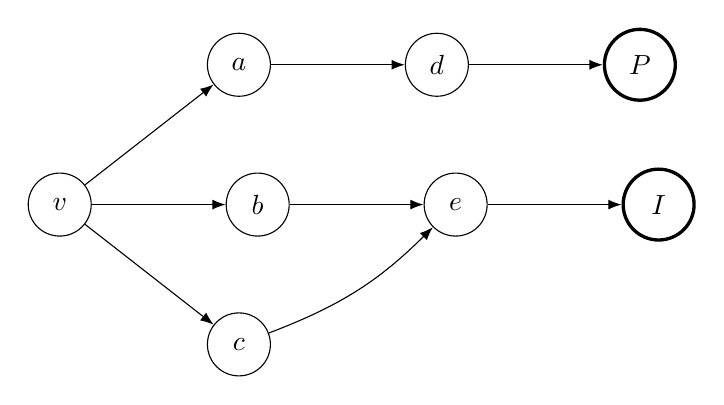
\begin{tikzpicture}[>=Latex,node distance=12mm and 17mm,
 state/.style={circle,draw,minimum size=8mm},term/.style={circle,draw,very thick,minimum size=9mm}]
\node[state] (v) {$v$};
\node[state,above right=of v] (a) {$a$};
\node[state,right=of v] (b) {$b$};
\node[state,below right=of v] (c) {$c$};
\node[state,right=of a] (d) {$d$};
\node[state,right=of b] (e) {$e$};
\node[term,right=of d] (p) {$P$};
\node[term,right=of e] (i) {$I$};
\draw[->] (v)--(a); \draw[->] (v)--(b); \draw[->] (v)--(c);
\draw[->] (a)--(d); \draw[->] (b)--(e); \draw[->] (c) to[bend right=12] (e);
\draw[->] (d)--(p); \draw[->] (e)--(i);
\end{tikzpicture}
\caption{A proof-ocean fork. The compass chooses among outgoing tunnels; only verifier-backed terminal vertices count as settlement.}
\end{figure}

\section{Exact distance to settlement}
\begin{definition}[Settlement distance]
For $v\in V$ define
\[
d_{\Cset}(v)=\min\{m\in\Nat:\exists v=v_0\to v_1\to\cdots\to v_m\in\Cset\},
\]
with $d_{\Cset}(v)=\infty$ if no directed path reaches settlement.
\end{definition}

On a solved retained DAG, $d_{\Cset}$ is computed exactly by reverse breadth-first search from the terminal vertices. It is therefore a trustworthy ground-truth label for training a navigator.

\begin{proposition}[One-step descent]
If $0<d_{\Cset}(v)<\infty$, there is $u\in\N^+(v)$ with
\[
d_{\Cset}(u)=d_{\Cset}(v)-1,
\]
and no outgoing neighbor has smaller distance.
\end{proposition}
\begin{proof}
Take a shortest path from $v$ to $\Cset$. Its first successor has a suffix of length $d_{\Cset}(v)-1$. A smaller value would contradict minimality of the original path. Any neighbor with distance below $d_{\Cset}(v)-1$ would likewise produce a shorter path from $v$.
\end{proof}

\section{The exact compass and its fixed point}
\begin{definition}[Exact compass]
Fix a deterministic tie-break. Define $N:V\to V$ by
\[
N(v)=v\quad(v\in\Cset),
\]
and for $v\notin\Cset$ choose
\[
N(v)\in\operatorname*{arg\,min}_{u\in\N^+(v)}d_{\Cset}(u).
\]
\end{definition}

\begin{theorem}[Compass fixed-point theorem]
Assume every considered vertex has finite directed distance to $\Cset$. Then
\[
\boxed{\operatorname{Fix}(N)=\Cset.}
\]
Moreover, for $v\notin\Cset$,
\[
d_{\Cset}(N(v))=d_{\Cset}(v)-1,
\]
so $N^{d_{\Cset}(v)}(v)\in\Cset$.
\end{theorem}
\begin{proof}
Every settlement vertex is fixed by definition. Every nonterminal vertex has an outgoing neighbor whose distance is exactly one smaller, and the compass selects a distance minimizer. Hence no nonterminal vertex is fixed. Iteration decreases the nonnegative integer distance by one until it reaches zero.
\end{proof}

This is the useful pairing of a halting/fixed-point set with a well-founded monotone ranking function. The fixed-point statement says where the dynamics stop; the ranking function proves that the exact compass cannot wander forever under the reachability hypothesis. Ranking functions are standard termination tools in program verification \cite{bradley2005,leike2014}.

\section{Learning the compass}
On a new proof ocean the true $d_{\Cset}$ is hidden. Let $\widehat d(v)$ be a predictor trained from solved DAGs. A learned compass is
\[
\widehat N(v)\in\operatorname*{arg\,min}_{u\in\N^+(v)}\widehat d(u).
\]
Features may include theorem/goal syntax, learned clause or tactic value, known mathematical landmarks, local settlement-density measurements, cross-agent transfer information, and the settlement tensor. Existing theorem-proving work provides precedents for learning from prior proofs and for predicting proof progress \cite{goertzel2019,huang2025,crouse2019}.

\begin{theorem}[Half-step robustness]
On a unit-edge graph, if
\[
\sup_v|\widehat d(v)-d_{\Cset}(v)|<\frac12,
\]
then every learned-compass choice is also a true distance-minimizing choice. Consequently the learned compass has the same fixed points and reaches settlement in the same number of compass moves as the exact compass.
\end{theorem}
\begin{proof}
At a nonterminal vertex with distance $m$, a true best neighbor has distance $m-1$, while every non-best neighbor has integer distance at least $m$. Uniform error below $1/2$ cannot reverse that one-unit gap.
\end{proof}

\section{Settlement direction versus settlement state}
A predictive field may satisfy
\[
F(v)=(F_P,F_R,F_I,F_C),\qquad F_k\ge0,\qquad \sum_kF_k\le1.
\]
These values answer a navigation question: which settlement basin currently appears promising? They must not be interpreted as partial certificates. The certifier still imposes the one-hot terminal rule. This distinction lets a compass use gradients or density information while preserving mutually exclusive settlement semantics.

\section{Benchmark implication}
For a solved DAG, compute exact $d_{\Cset}$ labels backward from verified terminals. At every historical fork, hide future information and ask the trained model to rank the available tunnels. The strongest evaluation is then counterfactual: let the learned compass control a fresh search and compare verified settlement cost against the identical search with compass guidance disabled. The retained data should include failed branches, timestamps, resource costs, agent identity, and verifier outcomes.

The first deliberately generous benchmark uses ten solved pre-Infinity Metamath proof DAGs as training material, forty-nine downstream theorem targets, and one hidden Infinity target under a base where Infinity is withheld. The special target must not be scored as independent merely because proof and refutation searches fail; a legitimate metatheoretic certificate is required.

\section{Conclusion}
On solved proof DAGs the ideal compass is simpler than an abstract notion of search promise: it is exact graph distance to a certified terminal set. That gives a measurable target for learning. Settlement density and the tensor can then be treated as features that help predict the hidden distance on new oceans. The central hypothesis is empirical: geometry learned from solved DAGs will rank productive tunnels well enough to reduce verifier-confirmed search cost on unseen targets.

\begin{thebibliography}{9}
\bibitem{bradley2005} A. R. Bradley, Z. Manna, and H. B. Sipma, ``Termination of Polynomial Programs,'' \emph{VMCAI}, 2005, pp. 113--129.
\bibitem{leike2014} J. Leike and M. Heizmann, ``Ranking Templates for Linear Loops,'' \emph{TACAS}, 2014, pp. 172--186. \url{https://arxiv.org/abs/1401.5338}
\bibitem{goertzel2019} Z. Goertzel, J. Jakub\r{u}v, and J. Urban, ``ENIGMAWatch: ProofWatch Meets ENIGMA,'' 2019. \url{https://arxiv.org/abs/1905.09565}
\bibitem{huang2025} S. Huang, P. Song, R. J. George, and A. Anandkumar, ``LeanProgress: Guiding Search for Neural Theorem Proving via Proof Progress Prediction,'' 2025. \url{https://arxiv.org/abs/2502.17925}
\bibitem{crouse2019} M. Crouse et al., ``A Deep Reinforcement Learning Approach to First-Order Logic Theorem Proving,'' 2019. \url{https://arxiv.org/abs/1911.02065}
\bibitem{metamath} N. D. Megill and D. A. Wheeler, \emph{Metamath: A Computer Language for Mathematical Proofs}. \url{https://us.metamath.org/downloads/metamath.pdf}
\end{thebibliography}
\end{document}
